\chapter{Introduction}
\label{ch:intro}
\section{Background}
% 2019年至2022年間,全球社會面臨嚴重特殊傳染性肺炎(COVID-19)的大流行。為了減少疾病的肆虐,世界各國政府與世界衛生組織(WHO)展開廣泛合作,以減少病毒的傳播。在這個全球衛生危機期間,對可靠信息來源和準確健康指導的需求不斷增加。然而,這些信息需求的激增與社交媒體平台上錯誤信息和虛假消息的快速傳播相互交織,導致公眾普遍困惑。

% WHO使用「infodemic」一詞來描述大流行期間錯誤信息的傳播\cite{b1}。他們強調此類錯誤信息對國家防疫政策的潛在威脅。對不正確或具誤導性信息的信任可能導致不良健康行為和不遵守健康政策,加劇大流行帶來的挑戰。

% 儘管COVID-19疫苗的分發有助於逐步控制大流行,但病毒仍然存在,出現了被稱為長期COVID的後感染症狀,至少有10%的感染者確認存在這些後果。此外,觀察到在初次康復後再次感染的案例,美國退伍軍人事務部的研究顯示,再次感染患者有較高的死亡率、住院率和發病後症狀的風險。

% 儘管COVID-19的即時威脅減弱,但與長期COVID和再感染相關的持續風險需要公眾對COVID-19相關政策和信息保持關注。隨著世界步入與病毒共存的後大流行時代,假消息和錯誤信息的挑戰依然存在。特別是與長期COVID和再感染相關的問題,對錯誤信息至關重要。因此,及時準確地識別和分類此類錯誤信息變得至關重要。
\subsection{Infodemic}
From 2019 to 2022, the global community faced the challenges posed by the 2019 coronavirus disease pandemic (COVID-19). In response, governments around the world and the World Health Organization (WHO) collaborated extensively to reduce the virus's spread. During this global health crisis, a growing demand for reliable information sources and accurate health guidance arose. However, the surge in these information needs overlapped with the rapid spread of misinformation and false news through social media platforms, leading to widespread public confusion.\\

The WHO used the term "infodemic"\cite{b1} to describe the spread of misinformation during the pandemic. They emphasized the potential threat that such misinformation posed to national epidemic prevention policies. Trust in incorrect or misleading information could result in adverse health behaviors and non-compliance with health policies, worsening the challenges of the pandemic.
\subsection{Long COVID and reinfection}
Although the distribution of COVID-19 vaccines contributed to the gradual control of the pandemic, the virus persisted, giving rise to post-infection symptoms known as long COVID, confirmed in at least 10\% of those who contracted the virus\cite{b2}. 
\begin{figure}
    \centering
    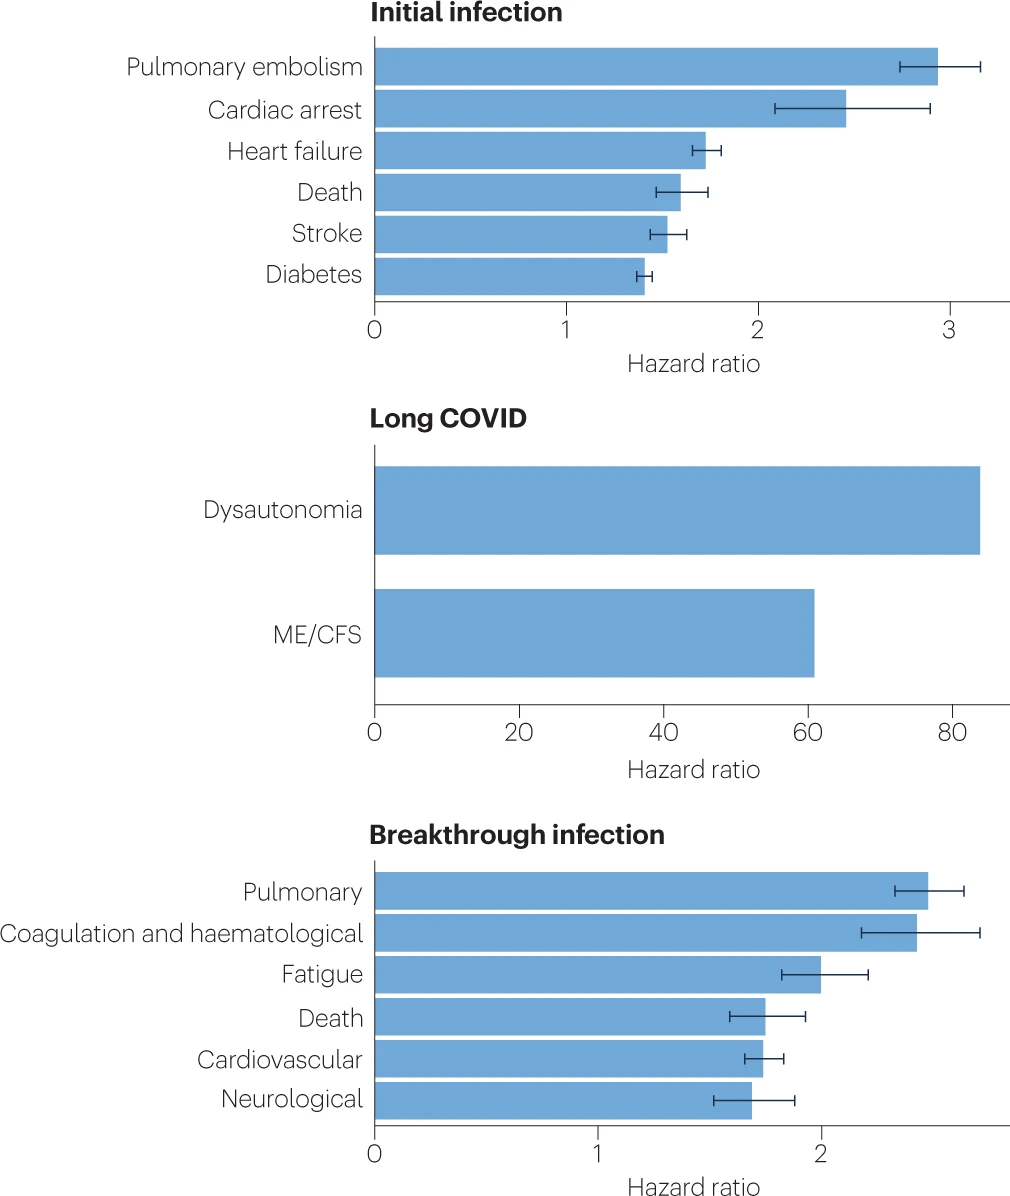
\includegraphics[width=0.75\linewidth]{img/long_COVID.png}
    \caption{The previous study revealed that COVID-19 and long COVID increases the risk of several medical conditions.\cite{b2}}
    \label{fig:long_COVID}
\end{figure}

Additionally, instances of reinfection after initial recovery were observed, with research from the US Department of Veterans Affairs indicating an increased risk of mortality, hospitalization, and postsymptomatic conditions in reinfected patients\cite{b3}.\\

Despite the diminishing immediate threat of COVID-19, the ongoing risks associated with long COVID and reinfection require public attention to COVID-19-related policies and information. The challenges of fake news and misinformation persist as the world transitions into a post-pandemic era coexisting with the virus. Specifically, issues related to long COVID and reinfection remain crucial to misinformation. Therefore, the timely and accurate identification and classification of such misinformation becomes critical.

\subsection{NLP techniques for fake news detection}
NLP techniques combine computational linguistic features and machine learning models to analyze and interpret human language comprehensively. By processing vast amounts of textual data, these techniques can distinguish linguistic patterns, semantic relationships, and sentiment analysis, promoting the identification of misleading content amidst genuine information.\\

Recent language models such as BERT (Bidirectional Encoder Representations from Transformers) and GPT (Generative Pre-trained Transformer) exhibit remarkable capabilities in understanding complex linguistic nuances and contextual meanings within sentences. These models use deep learning architectures to extract complicated semantic information, enabling them to distinguish between genuine and fake narratives effectively.\\

NLP plays an essential role in constantly fighting against misinformation by developing and adapting to emerging false information and linguistic patterns. These techniques help researchers and social platforms enhance the accuracy and efficiency of identifying the spread of fake news.

\section{Goal of This Study}
This study aims to investigate the performance of different deep learning models in detecting misinformation about long COVID. The objective is to develop a scientific and efficient method for identifying fake information in the context of long COVID in the post-pandemic era. Data related to long COVID misinformation were collected from open-source databases and through web crawling processes. These data then underwent a preprocessing phase to clean and refine the text in the dataset. After this, machine learning and various deep learning models were trained and evaluated based on their performance, following the preprocessing step. Additionally, the fuzzy rank-based ensemble approach was employed to combine the strengths of multiple models. Finally, the performance of this ensemble method was compared with the state-of-the-art large language models (LLMs) methods for detecting long COVID misinformation.

\section{Thesis Structure}
Chapter 2 reviews existing literature and previous studies related to fake news detection. It explores various approaches, methodologies, and techniques employed in NLP.
\\

Chapter 3, the method section, details our data collection, preprocessing, and training process. This includes an explanation of how we sourced data related to long COVID and reinfection misinformation from open-source databases and through web crawling. The chapter also discusses the preprocessing techniques we used to clean and refine the collected data, as well as the process of training various machine learning and deep learning models, and the workflow of the ensemble approach used to combine multiple models.
\\

Chapter 4 focuses on implementing the experiment based on the abstracted processes in Chapter 3. It provides insights into the tools, platforms, and technologies used to execute the research experiment effectively. Moreover, Chapter 4 also presents the experiment’s results, evaluating the proposed method’s performance in detecting long COVID misinformation and comparing it with state-of-the-art large language models (LLMs) methods.
\\

Finally, Chapter 5 discusses the principal findings, the implications of the results, and the limitations of the study.

